\documentclass[12pt,a4paper]{scrartcl}
\usepackage[english]{babel}
\usepackage[T1]{fontenc}
\usepackage[utf8]{inputenc}
\usepackage[color=yellow!15]{todonotes}
\usepackage{graphicx}
\usepackage[numbers, sort&compress, square]{natbib}
\usepackage[colorlinks, linkcolor=black, citecolor=blue, urlcolor=blue]{hyperref}
\usepackage{titlesec}
\usepackage{color}
\usepackage{booktabs}

% used for line numbering
\usepackage{lineno}

\makeatletter
\renewcommand\section{\@startsection{section}{1}{\z@}%
                     {-7.5ex \@plus -1ex \@minus -10.2ex}%
                     {2.3ex \@plus.2ex}%
                     {\sffamily\large\bfseries}}
\makeatother


\usepackage{geometry}
\geometry{a4paper, top=35mm, left=30mm, right=30mm, bottom=35mm,
headsep=10mm, footskip=12mm}

\title{\textbf{ \Large {Decentralized autonomous sensor fault detection using neural networks}}}
\author
{\large Katrin Jahr, Robert Schlich\\
\\
\normalsize{Degree program “Civil Engineering” (M.Sc.)}\\
\normalsize{Bauhaus-Universität Weimar, Germany}\\
\\
\normalsize{katrin.jahr@uni-weimar.de \qquad}
\normalsize{robert.schlich@uni-weimar.de}
}
\date{}

\clubpenalty = 10000 % schliesst Schusterjungen aus
\widowpenalty = 10000 \displaywidowpenalty = 10000% schliesst Hurenkinder aus 

\newenvironment{sciabstract}{%
\begin{quote} \itshape}
{\end{quote}}

\begin{document} 

% Double-space the manuscript.

\baselineskip20pt

% Make the title.

\maketitle 
\vspace{-2em}

% 
%\sloppy
\setlength{\emergencystretch}{3pt}
\hyphenation{sample-rate auto-nomous moni-toring methods}

\begin{sciabstract}

The dependability and the accuracy of structural health moni\-toring systems can be affected by sensor faults. 
In this paper, the design and implementation of a wireless structural health monitoring system, capable of decentralized autonomous fault detection, are presented. 
For self-detecting sensor faults, each sensor node predicts expected sensor data and compares it to the measured sensor data. 
The predictions are computed using neural networks based on measured sensor data of adjacent sensor nodes.
In laboratory experiments, devised to validate the proposed approach, several simulated sensor faults are detected.
These results indicate that the use of neural networks for fault detection increases the dependability and the accuracy of structural health monitoring systems.

\end{sciabstract}

%----------------------------------------------------------------------------------------

\linenumbers % Schaltet Zeilennummerierung ein
\modulolinenumbers[5] % nur jede 5. Zeile
\section*{Dictionary}

\begin{tabular}{|l|l|}
\hline 
Sensorknoten (SunSPOT) & sensor node \\ 
\hline 
einzelner Messsensor (Thermometer) & sensor \\ 
\hline 
Knoten im neuronalen Netz & neuron \\ 
\hline 
eine abgeschlossene Messungreihe & test run \\ 
\hline 
gemessene Werte & sensor data \\ 
\hline 
vorhergesagte Werte & predicted data \\ 
\hline 
durch Vorhersage erwartete Werte & expected data \\ 
\hline 
einzelner Messwert & measurement \\ 
\hline 
Test & laboratory experiments\\ 
\hline
tatsächliche, nicht virtuelle Messung & actual measurement \\
\hline
Messaufbau & test setup \\
\hline

\end{tabular} 

%----------------------------------------------------------------------------------------

\section*{Introduction}

Civil engineering structures are exposed to various external impacts during their lifetime. 
Structural health monitoring (SHM) systems can be deployed to evaluate the conditions and to ensure the structural stability of civil engineering structures.
\citet{BisbySHM} defines SHM as "a non-destructive \textit{in-situ} structural evaluation method that uses any of several sensors which are attached to, or embedded in, a structure".
The obtained sensor data is collected by sensor nodes, and then analyzed and stored on a computer system over long periods of time. 
The analysis of the sensor data can reveal abnormal changes in material and geometric behaviour at an early stage.

Traditionally, the sensor nodes are connected to computer systems with cables.
Using wired SHM systems has several disadvantages, including expensive wiring, high installation and labor costs as well as inaccessibility of optimal sensor location with wires.
In wireless SHM systems, the sensor nodes communicate---through a basestation with each other and with computer systems--- via wireless transceivers, eradicating wiring-specific problems.

Over their lifetime, sensors can become inaccurate, faulty, or may even break.
A fault can be defined as a defect of a sensor that leads to an error. An error is the manifestation of a fault---an incorrect system state---that may result in a failure.
To ensure the dependability and the accuracy of the SHM system, sensor faults must be detected and isolated in real time. 
A well known approach to fault detection is the installation of physically redundant sensors.
Faulty sensors can be identified through the deviation of their measurements from the measurements of correlated sensors.
Physical redundancy, although efficient for sensor fault detection, causes increased installation and maintenance costs due to the multiple installation of sensors. 
Representing a more efficient approach, analytical redundancy typically uses mathematical functions mapping the characteristics of the structure and the correlations of the installed sensors. Virtual sensor measurements are computed for each sensor and then compared to the actual measurements. 
For example, finite element models can be used in combination with data from adjacent sensor nodes to calculate virtual measurements of a sensor
\citep{Smarsly2014}.

In this study, analytical redundancy is implemented into wireless sensor nodes based on artificial neural networks.
Artificial neural networks essentially consist of interconnected data processing units called neurons. 
The neurons are grouped in different layers; usually one input layer, a number of hidden layers, and one output layer.
Artificial neural networks are able to learn, which is achieved by adjusting the weights of the inter-neuron connections until a set of given input variables results in the desired output variables; for example, a neural network can be trained to approximate any mathematical functions with any level of accuracy \citep{Li2011}.

This paper is organized as follows:
First, a wireless structural health monitoring system is designed and implemented. 
Next, a neural network is implemented into each sensor node and trained to predict the sensor measurements of the specific node for detecting sensor faults in a decentralized manner. 
Then, the system is tested in laboratory experiments. 
Finally, the experimental results are discussed and future research directions are proposed.

%----------------------------------------------------------------------------------------

\newpage

\section*{Design and implementation of the wireless structural health monitoring system}
In the following section, the wireless structural health monitoring system is introduced and the software implementation is described.
The wireless SHM system consists of wireless sensor nodes and a host computer, linked with a basestation.
The sensor nodes and the basestation are of type "Oracle Sun SPOT". 
The Sun SPOTS are equipped with several components.
Among others, the sensor board includes an accelerometer and eight independent RGB-LEDs.
The 3-axis digital output accelerometer with sensitivity ranging between $\pm$\,2\,g and $\pm$\,8\,g has a maximum sampling rate of 125\,Hz \citep{eDemo2010}.

The SHM system performs the following tasks:
1. data acquisition,
2. data processing,
3. data transmission, 
4. data storage,
5. diagnostics and 
6. information retrieval.
The dataflow is illustrated in \autoref{fig:flow}.
Tasks 1 to 3 are executed by the sensor nodes: During system operation, the sensor nodes acquire acceleration measurements and perform a FFT to determine the characteristics of the oscillation of the structure. 
The processed data is then transmitted via radio to the basestation and, finally, to the host computer.
On the host computer, tasks 4 is conducted by storing the data in a MySQL database.
Task 5 and 6---additional analysis and diagnosis---are conducted on the host computer in further steps.

\begin{figure}[htb]
    \centering
    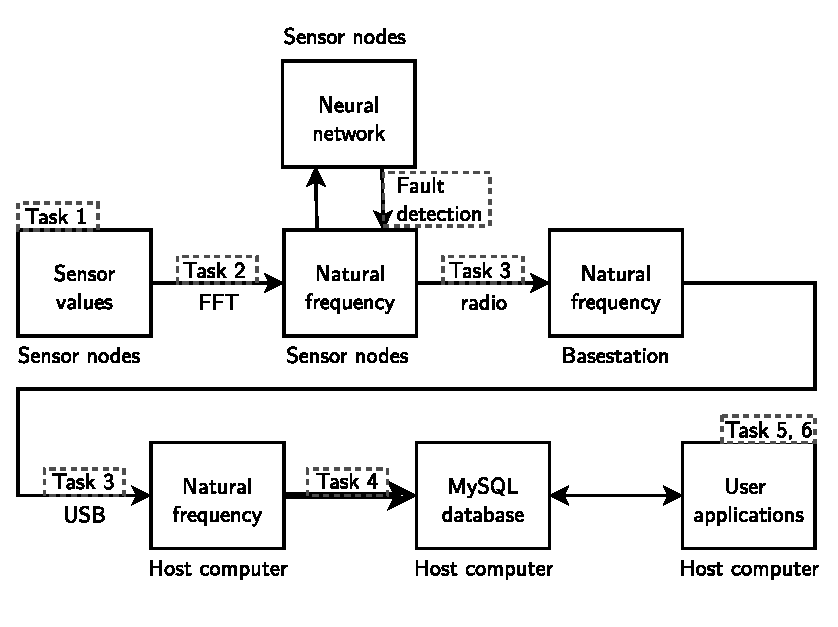
\includegraphics{figures/dataflow_tasks_nn.eps}
    \caption{Dataflow and associated SHM tasks}
    \label{fig:flow}
\end{figure}

\colorbox{cyan}{neuer Absatz:}
The SHM system is programmed object-oriented in Java. 
Object orientation uses objects, which are instanciated using classes as paradigm. 
A class includes methods, allowing the objects to perform actions, and attributes, storing object-specific data.
The SHM system consists of two packages---\texttt{sensornode} and \texttt{basestation}.
A package organizes several Java classes that build a program.

\autoref{fig:UML-sn} describes the classes of the \texttt{sensor\-node} package.
The package \texttt{sensor\-node} consists of the classes \texttt{Acceleration\-Sampler}, \texttt{FFT}, \texttt{Communi\-cation} and \texttt{Main\-Spot}, which are embedded directly into the sensor nodes.
The \texttt{Acceleration\-Sampler} class is responsible for measuring the acceleration.
There are two phases: \colorbox{cyan}{At} first, the acceleration is measured with a low sampling rate.
Once the acceleration exceeds a threshold, the \colorbox{cyan}{second phase is entered} by increasing the sampling rate. 
The measured values are stored into an array.
The different phases are indicatad by lighting different LEDs.
The \texttt{FFT} class performs a FFT on the measured accelerations. 
With the transformed data, the magnitudes and the correlating frequencies of the measured oscillation are calculated.
Finally, the natural frequency \colorbox{cyan}{is} determined by extracting the maximal magnitude.
The \texttt{Communi\-cation} class opens a radio connection between the sensor node and the basestation to transfer data from the sensor node to the basestation.
For starting the operation of \colorbox{cyan}{the sensor node}, the entry point of the programm is the \texttt{start\-App()} method in the \texttt{Main\-Spot} class. 
Within the \texttt{Main\-Spot} class, instances of the \texttt{Acceleration\-Sampler} class, the \texttt{FFT} class and the \texttt{Communication} class are created to perform the measurement.

\begin{figure}[htb]
    \centering
    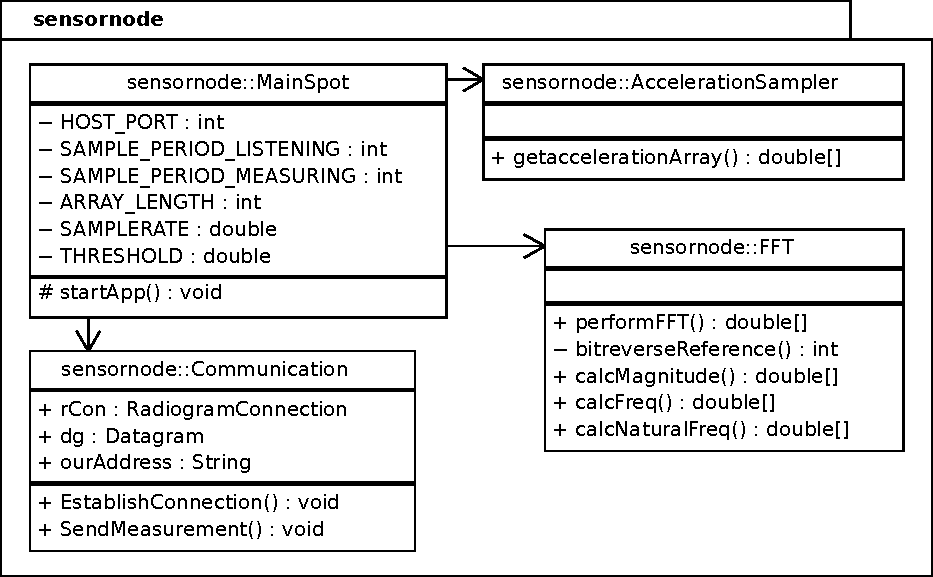
\includegraphics[width = \textwidth]{figures/uml-sensornode.pdf}
    \caption{Class diagram of the \texttt{sensornode} package}
    \label{fig:UML-sn}
\end{figure}

\autoref{fig:UML-bs} describes the classes of the \texttt{base\-station} package.
The package \texttt{base\-station} runs on the host computer and operates the basestation.
It consists of the classes \texttt{Database\-Handler} and \texttt{Main\-Base}.
The \texttt{Database\-Handler} class establishes a connection to a MySQL database, creates a database table, if none with the specified name is available, and inserts data into the database table.
The entry point of the program is the \texttt{run()} method in the \texttt{Main\-Base} class. The \texttt{Main\-Base} class opens a radio connection between the basestation and the sensor nodes, receives data sent by the sensor nodes and creates an instance of \texttt{Database\-Handler} to insert the data into the database.

\begin{figure}[htb]
    \centering
    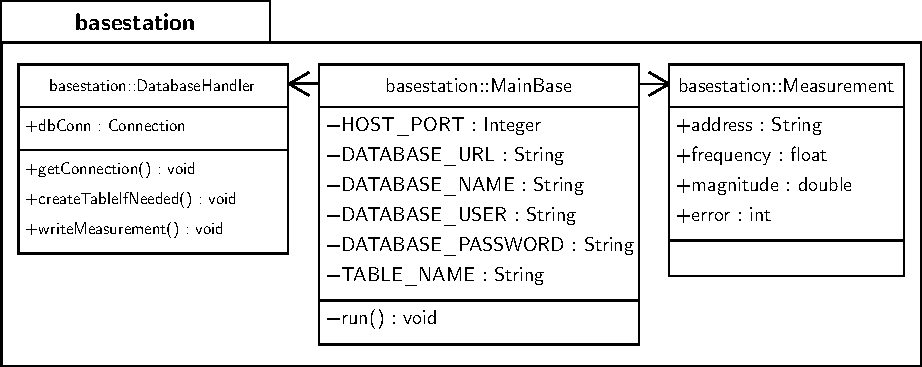
\includegraphics[width = \textwidth]{figures/uml-basestation.pdf}
    \caption{Class diagram of the \texttt{basestation} package}
    \label{fig:UML-bs}
\end{figure}

%----------------------------------------------------------------------------------------

\section*{Implementation and training of neural networks}

Neural networks are implemented into the sensor nodes using SNIPE, a open source Java Library.
\begin{figure}[ht]
    \centering
    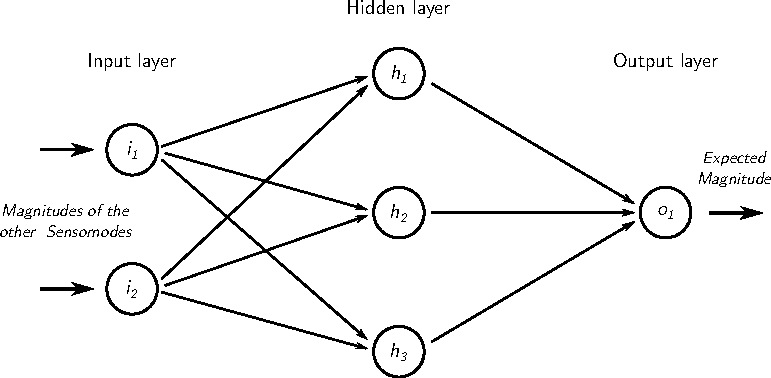
\includegraphics{figures/neuralnetwork.pdf}
    \caption{Schematic drawing of an artificial neural network with three layers}
    \label{fig:neuralnetwork}
\end{figure}
\todo[inline]{Grafik wird an unser neuronales Netz angepasst}


%\begin{itemize}
%\item neurons
%\item layer
%\item weights
%\item activation function / identity function
%\end{itemize}

%\textbf{2. paragraph: proposed nn}
%
%\begin{itemize}
%\item SNIPE? implementation in java?
%\item activation function / identity function
%\end{itemize}
%
%\textbf{3. paragraph: learning general}
%
%\begin{itemize}
%\item set with test values
%\item iterative weight adjustment
%\end{itemize}
%
%\textbf{4. paragraph?: learning, proposed}

%----------------------------------------------------------------------------------------

\section*{Laboratory experiments}

In the following section, the laboratory experiments are described.
First, a description of the test setup is given, second, the data aquisition and processing are depicted, and finally, the results are discussed. 

To validate the proposed approach in laboratory experiments, the wireless SHM system is installed on a test structure.
The test structure is a 4-story shear-frame consisting of four steel plates of 25\,cm\,$\times$\,50\,cm\,$\times$\,0.8\,mm.
The plates are mounted on threaded rods with a vertical clearance of 23\,cm.
At the bottom, the rods are fixed into a solid block of 40\,cm\,$\times$\,60\,cm\,$\times$\,30\,cm.
The SHM system is installed on the test structure by fastening one wireless sensor node to each of the top three stories.
The laboratory setup is shown in \autoref{fig:teststructure}.

\begin{figure}[ht]
    \centering
    \includegraphics[scale=0.4]{figures/testsetup.png}
    \caption{Laboratory setup (Source: own photograph)}
    \label{fig:teststructure}
\end{figure}

The structure is excited by deflecting and releasing the top of the structure.
This excitation method ensures a free vibration in natural frequency with little interferences.
After excitation, when the acceleration threshold is exceeded, the sensor nodes automatically start measuring the acceleration.
To minimize the wireless data traffic, each sensor node performs a FFT, once sufficient acceleration measurements have been collected.
By the use of the FFT, the acceleration measurements are converted into the oscillation frequencies and the corresponding magnitudes of the building \cite{rao2011fast}.

The implementation of the FFT has been verified by plotting the frequency domain of various oscillation events, see \autoref{fig:76hzfft}.
The natural frequencies can be identified by the peaks in the magnitude graph.
The first two natural frequencies are located at approximately 2.3\,Hz (1\textsuperscript{st} natural frequency) and 8\,Hz (2\textsuperscript{nd} natural frequency).
Each sensor node transfers the values of the first natural frequency and the corresponding magnitude to the basestation. 
The values are stored in a MySQL database and analyzed.

\begin{figure}[htb]
    \centering
    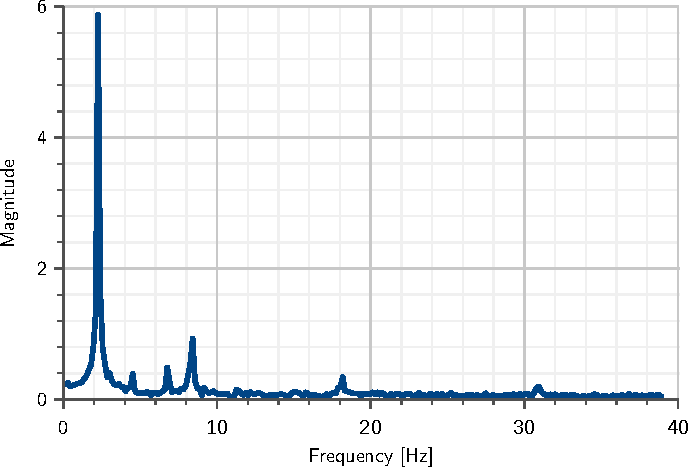
\includegraphics[scale=0.9]{figures/76HzHalf.pdf}
    \caption{frequency domain graph of the oscillation}
    \label{fig:76hzfft}
\end{figure}

The natural frequencies have been validated by repeated tests---using varying excitation forces, varying sampling rates, and varying quantities of measured values---and the results of a FE analysis.
The highest possible sampling rate was determined at 76\,Hz.
Higher samping rates could not be handled by the sensor nodes.
Test runs with more than 512 measured values showed no significant increase in precision.
Therefore, a sampling rate of 76\,Hz and 512 measured values were chosen.

\textit{Every sensor calculated the same natural frequency to a precision of four decimal points regardless of sensor position and degree of excitation.
Example results are shown in \autoref{tab:lab-ex}.
The identified magnitudes increase with ascending sensor node position from top to bottom, corresponding to the higher deflection at the top of the structure.}

\textit{Through FFT analysis of sampling events, the data traffic is decreased from 512 doubles per sampling event to two doubles per sampling event.
A number stored in the used data format double occupies 8\,bytes of space.
The data traffic is decreased by (512$-$2)$\times$8\,B\,=\,4080\,B\,=\,3,98\,MB per sampling event, decreasing data traffic by 99.6\,\%.}


\begin{table}[hb]
	\centering
	\begin{tabular}{l l c c c}
		\toprule
		ID & Position & Magnitude & Natural frequency [Hz] & Sampling rate [Hz]\\ 
		\midrule
		1 & top & 3.78 & 2.2461 & 76\\ 
		1 & middle & 3.23 & 2.2461 & 76\\ 
		1 & bottom & 1.97 & 2.2461 & 76\\ 
		\midrule	
		2 & top & 5.74 & 2.2536 & 76\\  
		2 & middle & 4.38 & 2.2536 & 76\\ 
		2 & bottom & 2.55 & 2.2536 & 76\\
		\midrule
		3 & top & 8.20 & 2.2536 & 76\\
		3 & middle & 6.35 & 2.2536 & 76\\ 
		3 & bottom & 3.79 & 2.2536 & 76\\
		\bottomrule
	\end{tabular}
	\caption{Natural frequencies of the test structure}
	\label{tab:lab-ex}
\end{table}

%----------------------------------------------------------------------------------------

\section*{Summary}

This paper has shown a decentralized autonomous sensor fault detection strategy for structural health monitoring systems based on neural networks. 
Autonomous sensor fault detection has been realized by implementing a neural network into each sensor node.
The neural networks have been trained to predict expected sensor measurements to be compared to actual measurments, in order to detect sensor faults.
The SHM system has been verified with laboratory experiments, proving that sensor fault detection using neural networks can improve the dependability and the accuracy of structural health monitoring systems.

%----------------------------------------------------------------------------------------

\bibliographystyle{unsrtnat}
\bibliography{literature}

\end{document}
